\section{Trusted Execution and Evidence Integrity}\label{sec:trust}

An \NDO{} verdict is only as trustworthy as the evidence behind it. The program under test runs inside the analysis and could, deliberately or accidentally, interfere with the observations from which the verdict is derived. This section states the threat model, the mechanisms and the residual risk. Section~\ref{sec:results} reports the adversarial evaluation (RQ1).

\subsection{Threat Model}
We consider three adversaries (Fig.~\ref{fig:threat}).
\begin{enumerate}
\item[A1)] \emph{An adversarial program under test}: Python code running in the evaluated process, with the analysis's user identity, inside the operating-system sandbox. It may patch the harness, write to or close file descriptors, terminate abruptly, or try to sense whether it is being analysed and behave differently.
\item[A2)] \emph{A keyless post-hoc writer}: a party that can modify files in the evidence directory after the run, including recomputing hash chains, but cannot read the controller's anchor key.
\item[A3)] \emph{An evidence substituter}: a party that replaces a pair's evidence with genuine evidence produced for a different program.
\end{enumerate}
Out of scope are holders of the anchor key (including any process running as the controller user that can read it), host, kernel or sandbox-runtime compromise, native-code attacks on the in-process harness, side channels, and sandbox escape. We make no claim of isolation against arbitrary adversarial programs.

\begin{figure*}[!t]
\centering
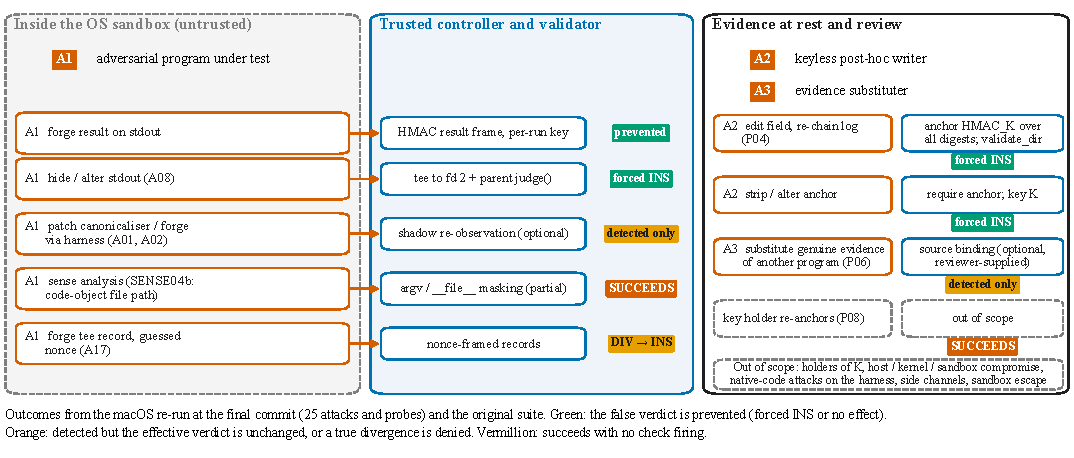
\includegraphics[width=\textwidth]{figures/fig_threat_model.pdf}
\caption{Threat model and outcomes. Each attack surface (left of each zone) is connected to the mechanism that addresses it and the outcome measured in the adversarial evaluation (macOS, final commit). Dashed elements are out of scope.}
\label{fig:threat}
\end{figure*}

\subsection{Mechanisms}
\paragraph*{Process roles} The \emph{controller} runs the unmodified V7-B runner, holds the anchor key and a session nonce, and never executes evaluated code. Each run of $P$ or $P'$ is an \emph{evaluated process}: a fresh child in its own process group with CPU, file-descriptor, file-size and core-dump limits; a resident-memory watchdog; a wall-clock timeout; an allow-listed environment that excludes the key; and an operating-system sandbox. On macOS the sandbox is a \code{sandbox-exec} profile that denies network access and confines writes to a working directory. On Linux it is \code{bwrap} with a read-only root bind, a writable working directory and network unsharing, or \code{unshare --net} as a fallback. The implementation applies no PID, user or IPC namespace, no seccomp filter and no cgroup limit, and it invokes no container runtime.

\paragraph*{Authenticated result channel} The child returns its result as a frame authenticated with HMAC-SHA256 under a fresh per-run key, passed over a pipe that is closed before user code starts. Standard output is never treated as protocol.

\paragraph*{Independent capture} The predecessor's harness captures standard output inside the evaluated process, where the program can tamper with it. \sbg{} interposes a stub that tees every write to the real file descriptor~2 as a nonce-framed record before the harness sees it. The controller compares these records with the harness's report. A mismatch, a missing record or a foreign record marks the run untrusted. Because the tee shares the evaluated process's address space, a program that replaces the output stream object itself, or reads the per-run nonce and forges consistent records, is not detected. This is a documented limit.

\paragraph*{Sealing and validation} Algorithms~\ref{alg:acquire} and~\ref{alg:validate} seal and validate the evidence directory. Only the validator feeds $\iota(\Ev)$ and hence the trust gate.

\paragraph*{Optional reviewer checks} Three checks report issues without changing the verdict:
\begin{itemize}
\item \emph{shadow re-observation} re-executes the pair with an independent minimal runner and canonicaliser in the sandbox and compares return values;
\item \emph{source binding} compares recorded program digests against sources supplied by the reviewer;
\item a \emph{pinned log head} is supplied out of band.
\end{itemize}
These checks provide \emph{detection}. They do not \emph{prevent} a false verdict unless a reviewer acts on them.

\subsection{Outcome Categories and Residual Risk}
An attack is \emph{blocked} if the effective verdict is forced to \INS{} by the engine or the trust gate. It is \emph{detected} if some check fires, \emph{without effect} if the true verdict is preserved, and \emph{successful} if a false or altered verdict results with no check firing. A detection by an optional reviewer check leaves the effective verdict unchanged, and we report it as \emph{detection only}. A blocked attack that turns a true \DIV{} into \INS{} denies a true divergence rather than creating a false assurance, and we report it separately. Table~\ref{tab:threats} maps each threat to its mechanism, the evidence and the residual risk.

\begin{table*}[!t]
\caption{Security threat summary: threat, mechanism, measured outcome and residual risk. Outcomes are from the macOS re-run at the final commit unless stated otherwise.}
\label{tab:threats}
\centering
\scriptsize
\setlength{\tabcolsep}{3pt}
\begin{tabular}{|c|L{3.3cm}|L{3.4cm}|L{3.6cm}|L{4.6cm}|}
\hline
Adv. & Threat (attacks) & Mechanism & Measured outcome & Residual risk \\
\hline
A1 & Forge a result on standard output (A06); exit early, write garbage to or close the result fd (A03--A05) & HMAC result frame, per-run key & A06 no effect; A03--A05 blocked (\INS{}) & None observed \\
A1 & Hide or alter standard output (A08) & Tee to fd~2, parent-side \code{judge} & Blocked (\INS{}) & Stream-object replacement or nonce reading in-process is not detected \\
A1 & Patch canonicaliser, forge via harness (A01, A02) & Shadow re-observation (optional) & Detection only; false \NDO{} remains effective & Requires reviewer action \\
A1 & Sense the analysis (SENSE01, 04, 04b--d; A07, A07c) & Masking of \code{\_\_file\_\_}, \code{sys.argv}; shadow (optional) & SENSE01, 04, 04d, A07c no effect; 04c and A07 detection only; 04b \emph{succeeds} & Code-object file paths reveal analysis; anonymised file names not implemented \\
A1 & Forge tee record with guessed nonce (A17) & Nonce-framed records & Detected; true \DIV{} becomes \INS{} & Denial of a true divergence \\
A2 & Edit a field and re-chain the log (P04) & Anchor $\mathrm{HMAC}_K$; validator & Blocked (\INS{}) & None for keyless writers \\
A2 & Strip or alter the anchor & Anchor required when key configured & Blocked (\INS{}) & Legacy directories without capture are not counted as untrusted \\
A3 & Substitute another program's genuine evidence (P06) & Source binding (optional) & Detection only & Requires reviewer-supplied sources \\
-- & Key holder re-anchors (P08) & Out of scope & Succeeds by design & Key management is outside the threat model \\
A1 & Linux isolation probes (74, pre-fix) & \code{bwrap}, network unsharing & 8 no effect; 1 succeeded (SENSE04); 65 \INS{}, cause unrecorded & Undecided runs are not evidence of isolation; no Linux re-run after remediation \\
\hline
\end{tabular}
\end{table*}
